\section{WS7: Truetime MATLAB Toolbox}
\label{section:truetime}

A computer network refers to a number of computers (also known as nodes) connected by some communication lines. These nodes can be any device that can be connected to a communication line, i.e: computer, sensors, switches, routers, etc.\\

The network is used for exchange information between nodes and some important applications regard the distributed systems where information and tasks are distributed to the nodes of the network.\\


QoS refers to traffic control mechanisms that seek to either differentiate performance based on application or network-operator requirements or provide predictable or guaranteed performance to applications, sessions or traffic aggregates. It specifies delay, delay variation (jitter), throughput (rate of sending data), error rate (packet loss).

Qos refers to network delays and packet loss. Qos is essential for time-critical applications such real-time control. 

In truetime the network is simulated as a shared broadcast link. Nodes are connected to a single line of communication and pairs of nodes use the line for a short time, the rest of nodes ignore it. The bus protocol is a distributed protocol used to decide who uses the link.\\
Despite being the standard for small networks, the bus topology has one drawback which makes the subject for the simulation: if the communication line experiences delays and information loss, the entire network is affected.



A queuing model is represented by a queue to which packets arrive, called arrivals, are being serviced and leave the queue. It is assumed that the arrivals and service follow a certain distribution. There are 2 types of queuing models: single server (), multiple server. Both model can use a finite queue lenght or an infinite queue lenght. An infinite lenght allows all packets to be serviced. A finite queue restricts the number of packets to be services and drops the rest. There can also be a finite or infinite population number. If a queue model is characterised by a Poisson distribution, then the arrival rate is $\lambda$. The service is following an exponential distribution at a rate of $\mu$. Due to the fact that the Possion distribution has an important feature, memoryless, a performance relation between the Poisson and exponential distribution can be drawn. It is important then that the ratio $\frac{\lambda}{\mu}<1$ meaning that the rate at which the packets are serviced is higher than the arrival rate if the length of the queue is infinite. It is assumed as well that the queue discipline follows a FIFO order.\\

If an infinite population is assumed, the queuing models are: single server infinite queue lenght ($M/M/1:/\infty/\infty$), single server finite queue lenght (), multiple server infinite queue lenght (), multiple server finite queue lenght (). The models use Kendall's notation for denoting a queuing node, i.e $M/M/1:/\infty/\infty$ - first $M$ stands for memoryless property of arrivals, second $M$ for memoryless of service, $1$ refers to the number of servers, and the last two infinity symbols stand for infinite queue lenght and infinite population number respectively. Being a memoryless model, the server has no state, it does not calculate the current state based on previous states because it has no memory of the previous states. 





This project develops a real-time control strategy for two Crazyflie quad-rotors connected to a ground station through a radio link. The ground station is connected to an Optitrack server communicating over Ethernet. A network view of the system is shown in Figure \ref{figure:system_design}.

\begin{figure}[H]
\centering
 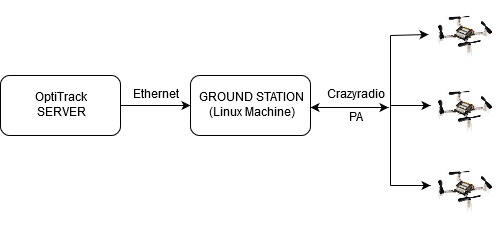
\includegraphics[scale=0.5]{Figures/crazyflie_system.png}
 \caption{A network view of the system design.}
 \label{figure:system_design}
\end{figure}

Usually controllers are developed and connected to other parts of the systems (nodes) over a network with different access protocols \cite{truetime}: wireless, CAN, Ethernet, etc. Although delays and information loss occurs in the network, controllers may not be developed to overcome the effects of these network constraints. It is often assumed that there is enough computing power and a fast and reliable communication network. When simulating the controller of a plant it is important to simulate the network model and its influence on the controller so the plant can overcome disturbances coming from the network.\\


Truetime (tt) is a MATLAB/Simulink toolbox for simulation of distributed real-time control systems. It mainly consists of Truetime kernels substituting for computer nodes in the network and Truetime network interfaces (wired, wireless and ultrasound). The plant process and controller can be designed in Simulink and connected with ttkernels and ttnetworks. Controllers however can be designed as a ttkernel or imported from an already existing Simulink block.
The ttkernels and other blocks can be accessed from the ttlibrary by typing in Matlab command line $trutime$ and the blocks can be programmed by using m-files. The ttlibrary allows to simulate discrete network controllers \cite{chvostek2007simulation}.\\

The simulated environment aims to be as close to the real system as possible. The main components of the real system in Figure \ref{figure:system_design} are the ground station, the server (Optitrack) and three Crazyflie of which only 2 are used for experiments. In the simulation there are 2 nodes: the ground station (GS) node and the communication node. The GS node acts as a server sending messages to the communication node with commands for the internal controller of the Crazyflie. The server node is also the position controller which runs offboard and gives [x y z yaw] coordinates to the drones. Hence this ttkernel is the PID discrete controller. The communication node is a ttkernel that receives and sends network messages and is referred to as the client. The actual x position represents the Optitrack measurements in the real system which is connected to the ground station by an Ethernet/wired connection. The Optitrack system is replaced in the simulation by the actual calculated x position. The Crazyflie is simulated as an attitude controller using Simulink. It receives the PID commands from the controller through the client node and outputs the calculated position which is fed back into the controller. This structure can be seen in Figure \ref{position_contr_simulink}.\\

\begin{figure}[H]
\centering
 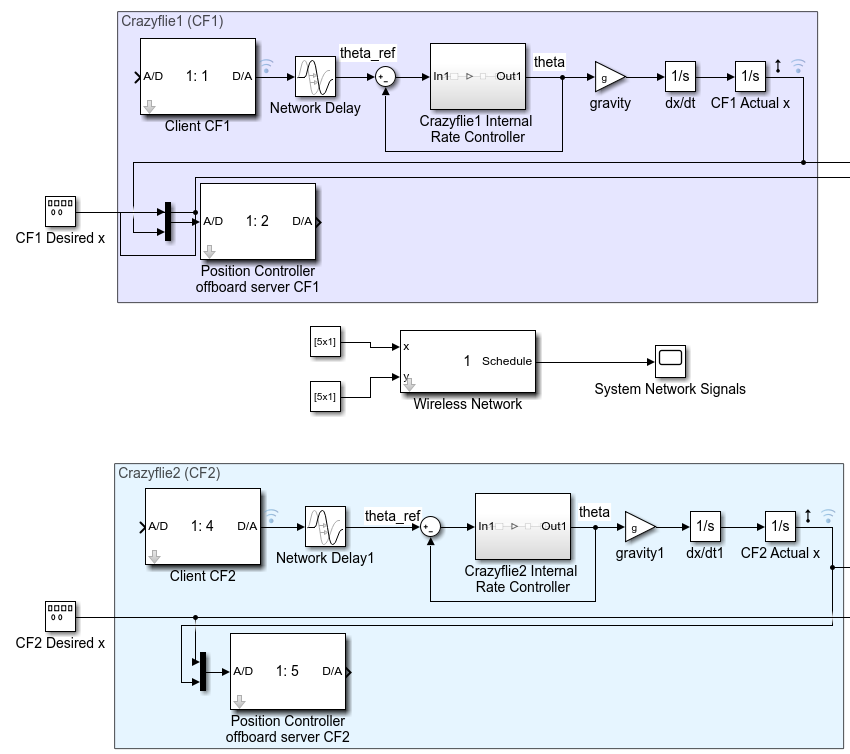
\includegraphics[scale=0.6]{Figures/position_contr_sim.png}
 \caption{The simulated position controller on the x-axis using Truetime kernels.}
 \label{position_contr_simulink}
\end{figure}

Asserting from Figure \ref{figure:system_design} there are two network types in the system: Ethernet and radio (2.4GHz). 

\begin{figure}[H]
  \centering
    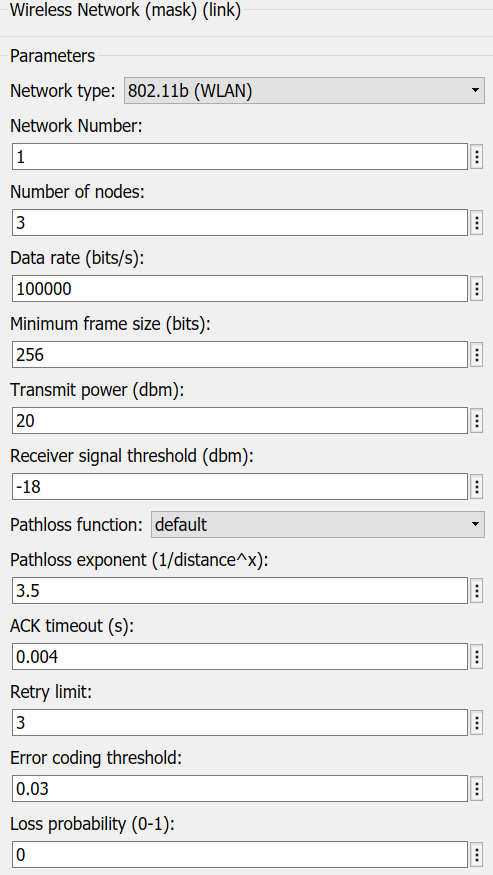
\includegraphics[width=0.5\textwidth]{Figures/network_interf.png}
  \caption{The wireless ttnetwork interface using Crazyflie's Radio AP specifications.}
  \label{figure:network_inter}
\end{figure} 

The radio connection between the ground station running the position controller and the Crazyflie is of interest to be simulated. A wireless network interface is added to the simulation to be carrying the messages between the 2 ttkernels: position controller and client. The interface carries all specifications of the Crazyflie AP USB dongle: 

\begin{enumerate}
    \item Data rate: 250 kbps
    \item Minimum frame size: 512 bits
    \item Receiver signal threshold: -18 dbm
    \item ACK timeout: 0
    \item Retry limit: 0
\end{enumerate}

These can be seen in Figure \ref{figure:network_inter}. The data rate to be simulated is chosen at 250 kbps however the Crazyflie AP capabilities also includes a throughput of 2 Mbps. The 2 Mbps is recommended to be used in an environment with high interference. The Received Signal Strength Indicator (RSSI) is used to analyse the interference of the environment in the WNS lab. As a rule of thumb, the RSSI should be below 80 for a good network link \cite{book_ros}. The WNS lab is a high interference environment as the lowest RSSI read was 135 with an average RSSI of 200.\\ 

A wireless interface is considered to best simulate the real system in regards to sending of messages and receiving acknowledgement (ACK) from the drone back. In the real system and a perfect network there should be one ACK sent for one packet received. However since the network is not perfect, the packets sent are analysed using the Link Quality (LQ) ratio which is shown in Equation \ref{eq:lq}. 

\begin{equation} \label{eq:lq}
	LQ = \frac{ACK}{100}
\end{equation}


An LQ of 1 means that 100 ACKs have been sent per 100 packets. This transmission of ACKs is handled by the network ttkernel however in other network interfaces this feature is not supported and hence it has to be implemented to maintain resemblance to the real system. ACK timeout and retries add delays to the network and so have been set to 0. It is expected to have a lower average LQ on the 250 kbps network than the 2 Mbps. The pathloss exponent influences the quality of the network depending on the distance of the nodes - the further apart the nodes are the smaller the interference. In this system the nodes are not more than 1 meter apart. The coordinates of the nodes have been included as shown in Figure \ref{wireless_network}.


\begin{figure}[H]
\centering
 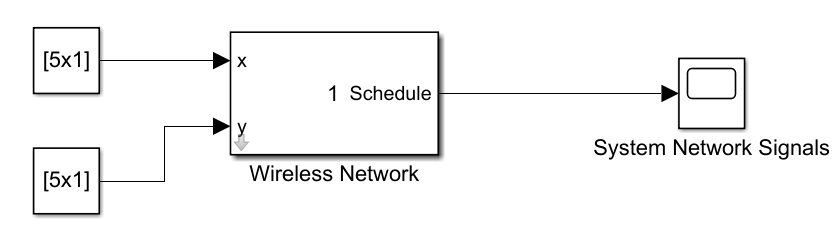
\includegraphics[scale=0.6]{Figures/wireless_network.png}
 \caption{The wireless ttnetwork interface connected to 5 nodes for which a vector of dimension 5x1 is required for the x-coordinate as well as the y-coordinate.}
 \label{wireless_network}
\end{figure}

On the network of the real system there are 3 drones connected to the ground station however the network analysis is done using 2 drones as one is used as backup. In order to simulate the same system, a second drone has also been added to the simulation. The final setup of the network simulation is shown in Figure \ref{position_contr_simulink}.


\begin{figure}[H]
\centering
 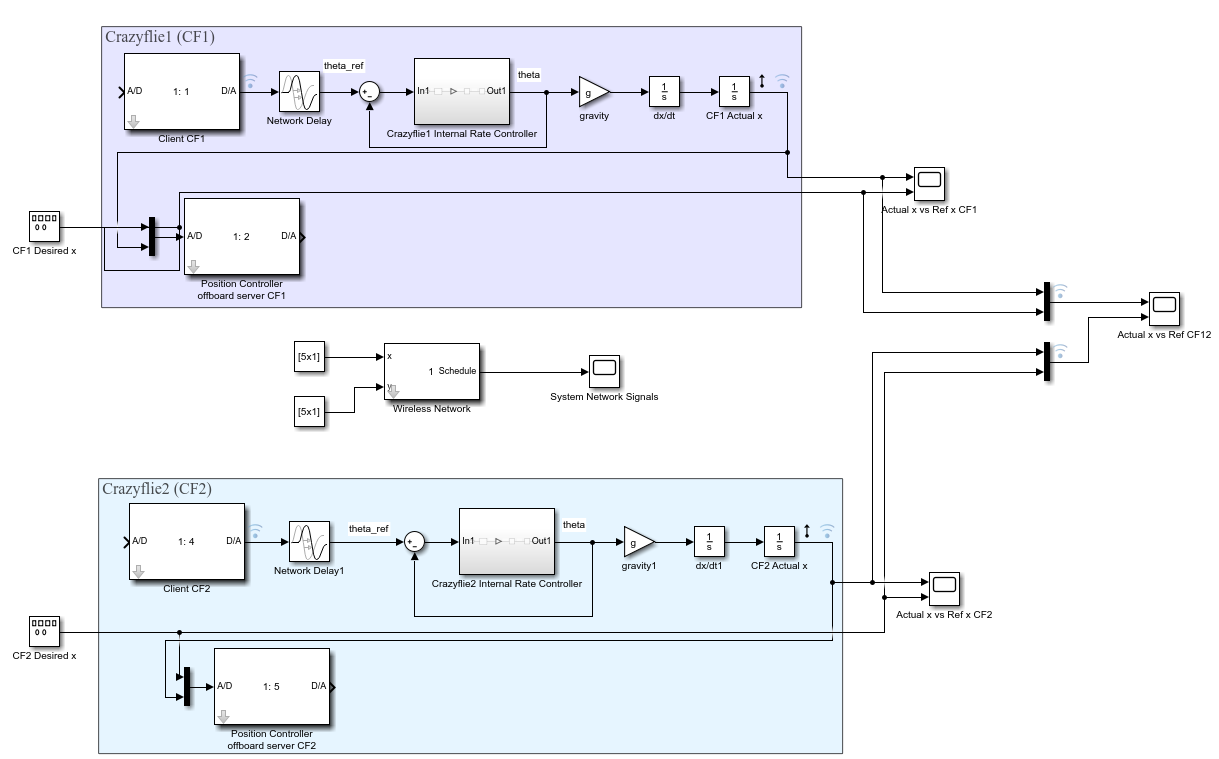
\includegraphics[scale=0.6]{Figures/network_simulation.png}
 \caption{The distributed real-time position controllers over 2 Crazyflies simulated using Truetime kernels. It simulates packet loss and network delay.}
 \label{position_contr_simulink}
\end{figure}

In order to simulate packet loss and network delay, a delay has been added between the client node sending the commands to the Crazyflie. Its task is to delay the messages transmitted simulating Crazyflie receiving updates position updates at a lower frequency than 50 Hz.\\  

%Its task is to transmit dummy messages on the network. The dummy messages transmitted follow a uniform distribution having the same 100 Hz frequency as the position controller. \\

Figure \ref{position_contr_simulink} shows the blocks of the Truetime simulation. The Ethernet network between the Optitrack server and the ground station is simulated as wired blocks in Figure \ref{position_contr_simulink}. It is assumed that this type of network has no delays or packet loss. The radio connection is simulated through the wireless network interface between the D/A output port of the Position Controller ttkernel to the A/D input port of the Client ttkernel.

Each kernel can have several A/D inputs and D/A outputs as well as network input/output defined by the $ttGetMsg$ and $ttSendMsg$ command. Each node in the network loop has clearly defined tasks:

\begin{itemize}
    \item Node 1/4 $Client$ (communication node):
    \begin{enumerate}
        \item Get message from network containing PID commands from node 2;
        \item Analog output the message received to the Crazyflie internal controller;
    \end{enumerate}
    \item Node 2/5 $Position$ $Controller$ (acts as controller/server):
    \begin{enumerate}
        \item Analog input(1) the message with actual position (calculated);
        \item Analog input(2) the reference position from the trajectory generator;
        \item Calculate error between reference and actual measurements;
        \item Calculate the PID commands;
        \item Send message over the wireless network to node 1;
    \end{enumerate}
    \item Node 3 $Wireless$ $Network$ $Node$ (wireless network node):
    \begin{enumerate}
        \item Send messages from node 2 to 1 and node 5 to 4;
        \item Introduce packet loss over the network.
    \end{enumerate}
\end{itemize}

Before tuning the position controller, it is necessary to ensure that the packets sent through the network are received by the nodes and that each node performs its task. This has been checked by displaying warnings when nodes received or did not receive any message. One issue observed at first was related to the controller node which had to send a message when it received another from the network. However, going up the chain the other node waits for the controller's message in order to send the message to the plant that sends the message back to the controller. This was displayed as a mismatch between the nodes as can be seen in Figure \ref{figure:success} using the Diagnostic Viewer in Simulink. The issue has been solved by making the client an aperiodic task to run continuously while the controller node is a periodic task triggered by the event of an incoming message on the network.\\

\begin{figure}[H]
\centering
 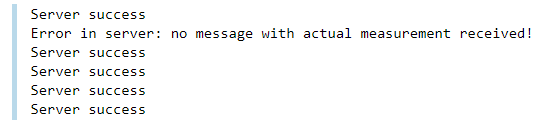
\includegraphics[scale=0.8]{Figures/diagnostic_viewer.png}
 \caption{Simulink Diagnostic Viewer showing the warning messages sent by the nodes as the network is simulated.}
 \label{figure:success}
\end{figure}

In the simulation the behaviour of the position controller on the x-axis is analysed. The Crazyflie internal attitude controller is created from the linearized equations of motion of the drone. It is important to note that Truetime simulates discrete controllers and hence the PID programmed in the Position Controller ttkernel is discrete using the formula given by Simulink. In order to correctly tune the discrete controller inside the network loop, a Simulink discrete position controller had to be created outside the network loop. Figure \ref{figure:discrete_controller} shows the position controller on the x-axis. The inner attitude controller is a continuous controller. 

\begin{figure}[H]
\centering
 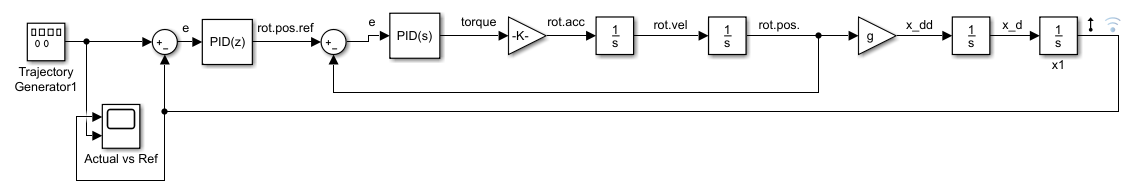
\includegraphics[scale=0.6]{Figures/pos_contr_simulink.png}
 \caption{The discrete position controller on the x-axis to be used in the network loop.}
 \label{figure:discrete_controller}
\end{figure}

Tuning the discrete controller using the Truetime recommended sample time to stabilise the system proved to be difficult. In fact, the system was unstable. Once the sample time has been changed to the sample time of the actual Optitrack server 100 Hz, the system became stable. It is a slow system to reach steady-state. The gains of the system are also low as can be seen in Figure \ref{figure:tuning_discrete}.

\begin{figure}[H]
\centering
 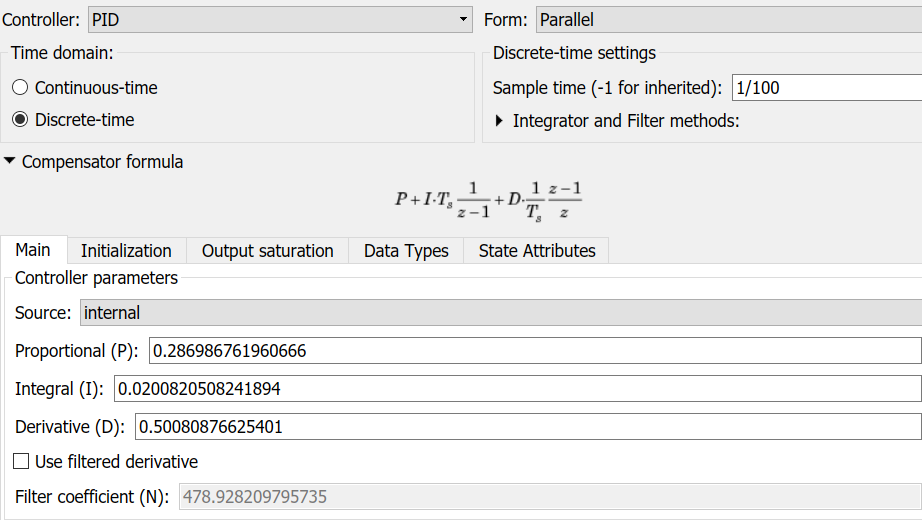
\includegraphics[scale=0.6]{Figures/tuning_discrete.png}
 \caption{The discrete controller gains, sample time and formula. The formula is used for the discrete position controller ttkernel in the network simulation.}
 \label{figure:tuning_discrete}
\end{figure}

Having the discrete controller tuned it is programmed as the Position Controller ttkernel. The ttkernels require one m-file to initialise called $controller\textunderscore init$, or $client\textunderscore  init$ respectively. The initialisation m-file of the controller kernel looks as shown in Listing \ref{listing:controller_init}.

\begin{lstlisting}[language=Matlab, caption={controller\textunderscore init.m}, label={listing:controller_init}]
% Distributed control system: controller node
%
% Receives messages from the sensor node, computes control signal
% and sends it to the drone.

data.h = 0.01;
data.KP = 0.286986761960666;
data.KI = 0.0200820508241894;
data.KD = 0.50080876625401; 
data.epsilon = 0;
data.error = 0;
data.old_error = 0;
data.u = 0;


% controller task activated by arriving network message
starttime = 0.0;
deadline = data.h;
ttCreatePeriodicTask('controller_task', starttime, deadline, 'controller_node', data);
ttAttachNetworkHandler('controller_task')
\end{lstlisting}

In the initialisation m-file all required data such as the gains, start time and period of the task, variable initialisations are defined. Lines 36 - 37 in Listing \ref{listing:controller_init} shows calling of the periodic task function which refers to another m-file where the $controller \textunderscore  node$ actual task resides. The task can be seen in Listing \ref{listing:controller_node}. The network handler $ttAttachNetworkHandler$ indicates that the controller task communicates messages over the network.

\begin{lstlisting}[language=Matlab, caption={controller\textunderscore node.m}, label={listing:controller_node}]
function [exectime, data] = controller_node(seg, data)

persistent y_r
persistent y_act
persistent old_error

switch seg
    case 1
        y_r = ttAnalogIn(1);
        y_act = ttAnalogIn(2);
        exectime = 0.0005;
    case 2
        data.error = (y_r-y_act);
        P = data.K*data.error;
        
        data.epsilon = data.epsilon + data.h*data.error;
        I = data.epsilon*data.KI;
        
        D =((data.error - data.old_error)*data.KD)/data.h;
        data.old_error = (y_r-y_act);
        
        data.u = P + I + D;
        exectime = 0.0005;
        
    case 3
        ttSendMsg(1, data.u, 256); % Send message (256 bytes) to node 1 (controller)
        ttAnalogOut(1, data.u);
        exectime = -1; % finished
end
\end{lstlisting}

In a similar way, the other kernels are initialised and defined. The Matlab code is listed under Appendix \ref{chapter:Appendix1}.\\

The wireless network interface displays the signals from all 4 nodes communicating through the network. Each pulse in the signal represents a message sent and that the network is busy. It is important that there are no message collisions, meaning that nodes do not transmit messages at the same time. The nodes which do not send any message on the network are the communication nodes namely $Client$ $CF1$ and $Client$ $CF2$. The interference node is placed to create background interference however it is not used in this simulation.

\begin{figure}[H]
\centering
 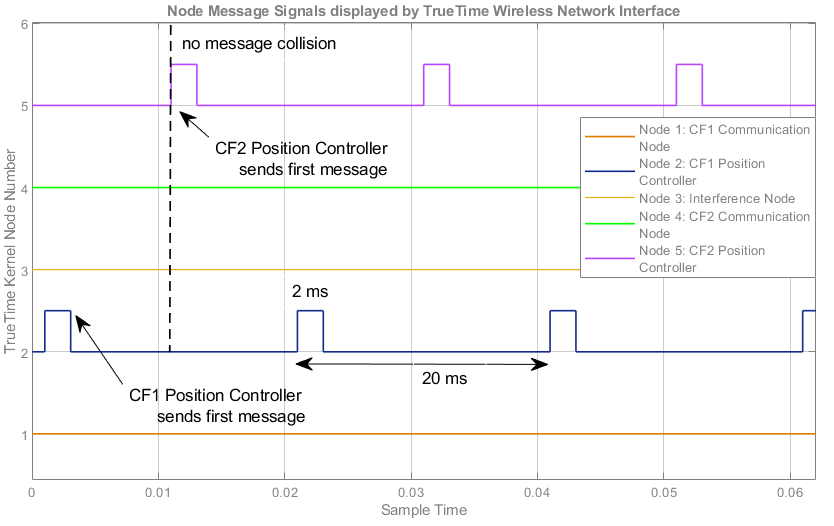
\includegraphics[scale=0.5]{Figures/network_inter0.png}
 \caption{The wireless network interface showing the signals of the nodes with no delay nor packet loss in the network. Each signal corresponds to a node in the simulation.}
 \label{figure:network_signal0}
\end{figure}

In Figure \ref{figure:network_signal0} the $Controller$ signals are shown with no packet loss nor delay. The signal has a frequency of 50 Hz. The resulting system behaviour with no interference can be seen in Figure \ref{figure:noloss}.

\begin{figure}[H]
\centering
 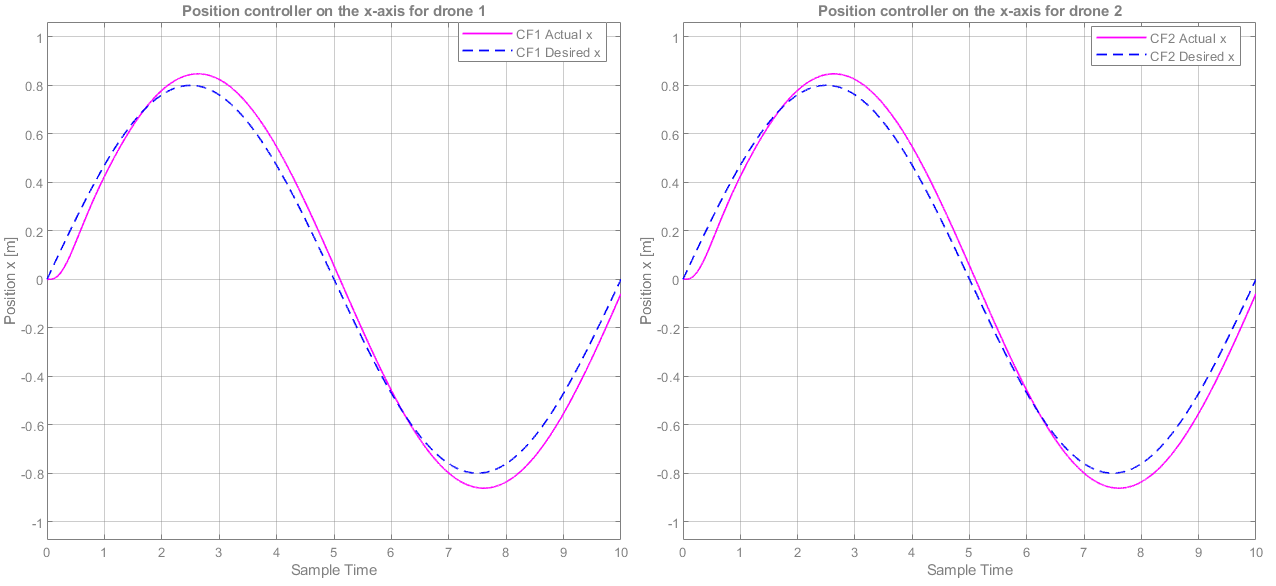
\includegraphics[scale=0.4]{Figures/2drones_noloss.png}
 \caption{The systems behaviour on the x-axis position controller of the two drones when there is no packet loss or delay in the network.}
 \label{figure:noloss}
\end{figure}

Adding delay to the network, it has been noticed that the system remains marginally stable at 0.23 seconds (s) delay meaning that the system can still be stable at 4 Hz. Considering that the rule of thumb for running position updates is 50 Hz, this result seems unrealistic. The system response to the delay can be seen in Figure \ref{figure:network_signal01}.

%Changing the argument of the interference node to use 15\% of the bandwidth using dummy messages, the network signal of the PID controller is affected with changes to the behaviour of the system, especially its stability. See Figure \ref{figure:network_signal01} for the network signal and Figure \ref{figure:loss01} for the system behaviour.

\begin{figure}[H]
\centering
 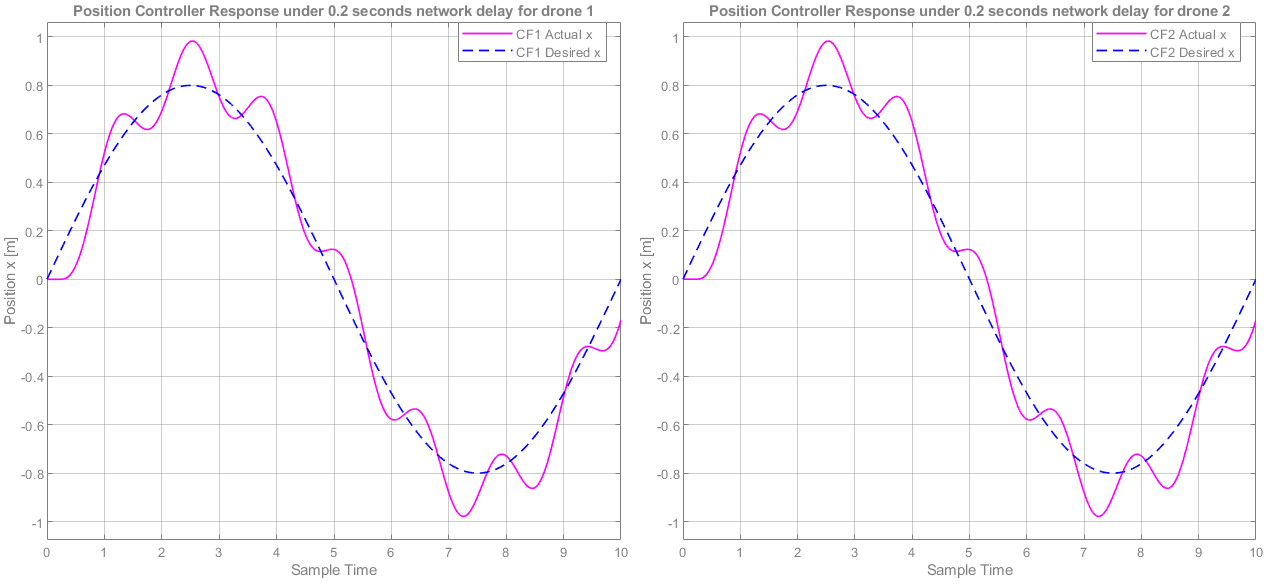
\includegraphics[scale=0.4]{Figures/2drones_2delay.png}
 \caption{The systems response of the two drones when a delay of 0.23 seconds is added to the network.}
 \label{figure:network_signal01}
\end{figure}

Adding packet loss probability to the network with no delay, the controllers of both drones remain stable to 90\% packet loss however at 91\% packet loss, controller of $CF1$ becomes unstable while controller of $CF2$ remains stable. At 92\% packet loss, both controllers become unstable. The controller have been observed to behave differently to other levels of delay and probability loss. The controllers response can be seen in Figure \ref{figure:loss01}.

\begin{figure}[H]
\centering
 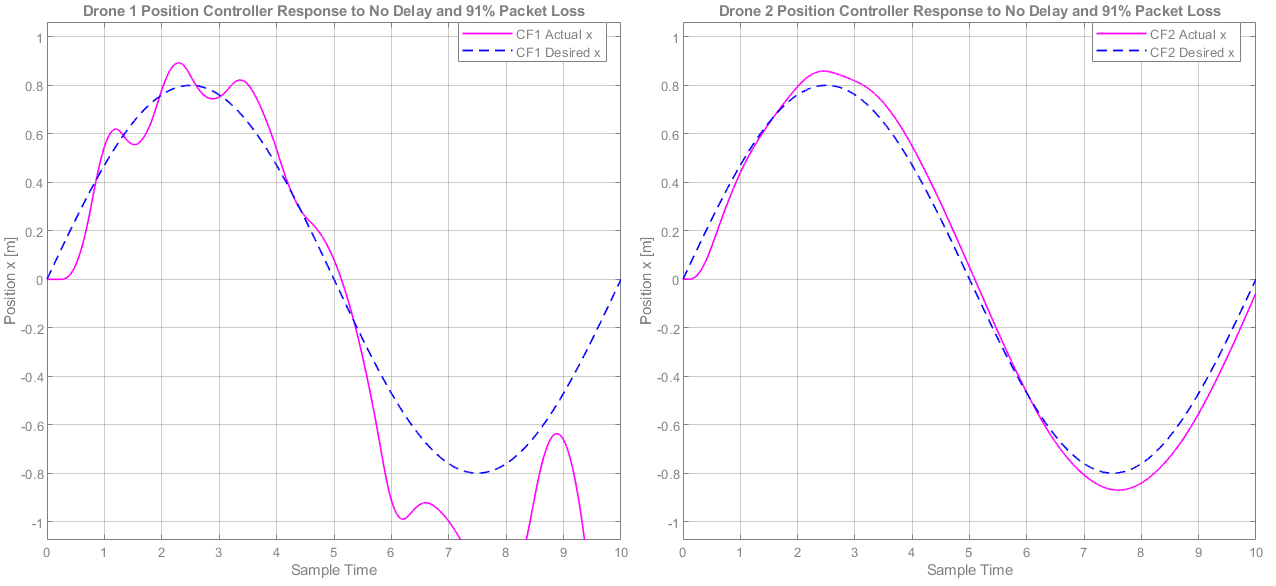
\includegraphics[scale=0.4]{Figures/2drones_91prob.png}
 \caption{The position controller of the two drones affected differently by 91\% packet loss with no delay in the network. The controller are both stable at 90\% packet and unstable at 92\%.}
 \label{figure:loss01}
\end{figure}

Having simulated of the two controllers at different levels of packet loss probability and delay resulted that the system remains marginally stable at a level of 0.36 probability of packet loss and 0.2 s network delay. Given that the system is composed of two drones, the reported level represents a critical limit that may render drones to behave unexpectedly. The system's response to the reported level can be seen in Figure \ref{figure:loss03}.

%A bandwidth of 10\% seems not to affect the system and can be considered as usable for a drone however at 15\% usage the system presents variations which may be unsafe for a drone even though the system seems to recover. While it may not crash, these variations can drive the drone outside Optitrack's range and crash due to the lack of positional data. The unpredictable behaviour of the system at 20\% bandwidth is shown in Figure \ref{figure:loss03}.

\begin{figure}[H]
\centering
 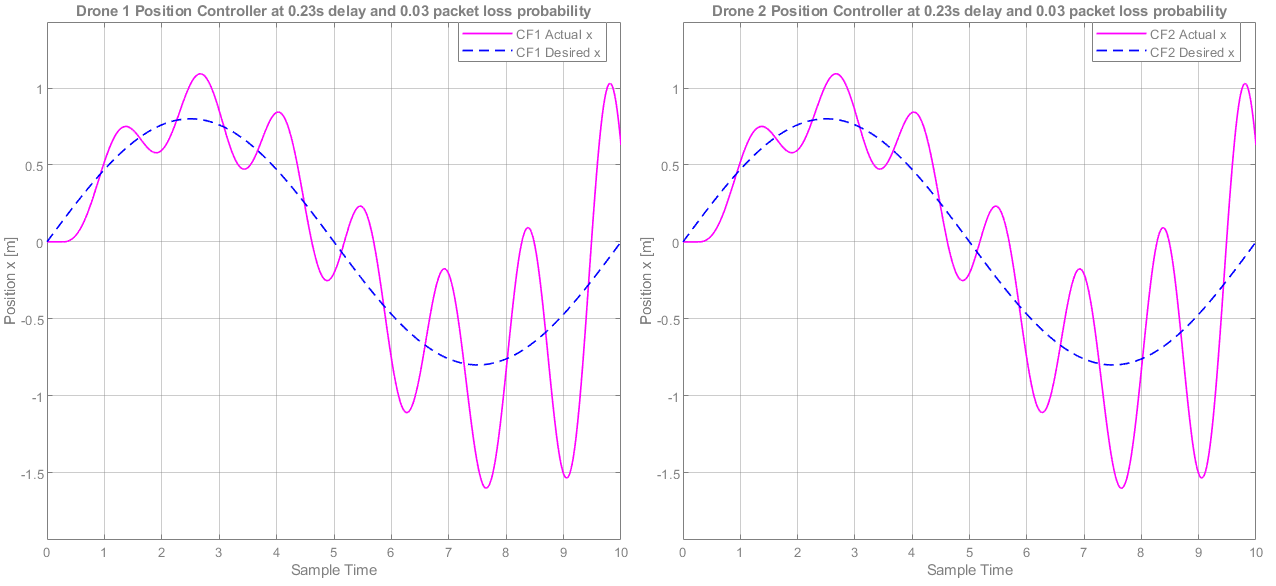
\includegraphics[scale=0.4]{Figures/2drones_maxprob.png}
 \caption{The position controller affected by 20\% bandwidth interference in the network. For an indoor flying drone this controller is considered unstable. }
 \label{figure:loss03}
\end{figure}

The simulations performed graph a controller stability curve for both drones with minor differences which are neglected. Similar experiments were run in parallel with two drone in hover mode. The experiments were investigating the network effects on the z-axis controller. However, even though the simulation was analysing the x-axis controller the delay found that would render the control unstable is 10 times higher compared to the delay found through experiments. The simulations found a network delay of 0.2 s and the experiments found a delay of 0.03 s up to which the drones remain stable. Even though the drones could hover even at 0.04 s delay there were high oscillations for small errors in position. Stability of the drones with delays higher than 0.03 s cannot be replicated. Converging all data gathered through the simulations and experiments, the controller stability curve given by the simulations and by the experiments can be seen in Figure \ref{figure:stability_curve}.\\

\begin{figure}[H]
\centering
 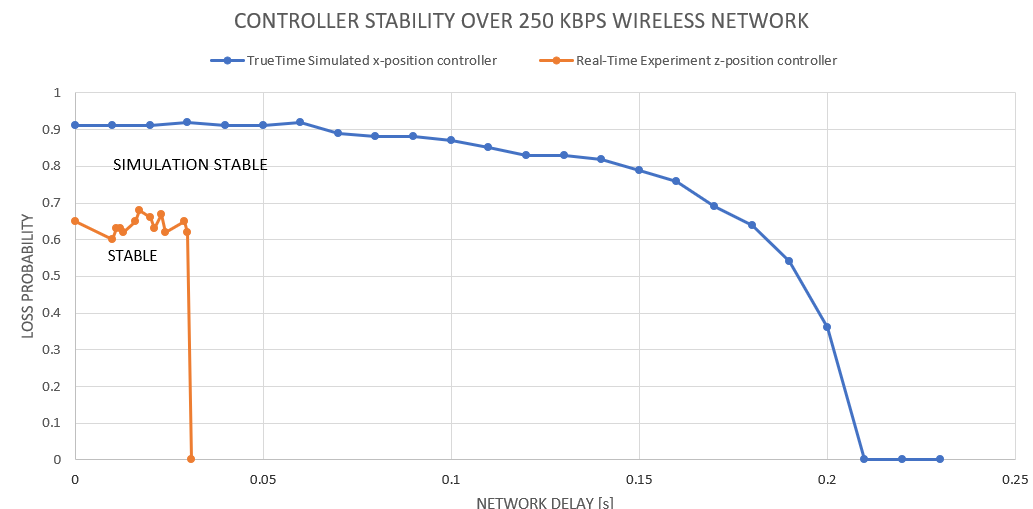
\includegraphics[scale=0.65]{Figures/controller_stability_line.png}
 \caption{The controller stability curves determined through simulations of the x-axis position controller and experiments of the z-axis controller. The area under the curve is considered a stable system.}
 \label{figure:stability_curve}
\end{figure}


\subsection{WS6: Discussion on other types of ttnetworks}

%____________________________________________________
The building blocks of a network is constituted by a protocol. A protocol has two interfaces: the service layer and the peer-to-peer interface. The service layer defines the operations of the protocol and the peer-to-peer interface defines the messages exchanged. Each layer performs a task which is a service to the upper layer as most networks are organised in a series of layers. Each task is performed using the peer-to-peer interface to the corresponding peer's layer.

The Optitrack server is designed as a broadcast type of communication link.
The communication link between the ground station and the Crazyflies is of type point-to-point, each node with its own channel.

% bandwidth is the range of a frequency.
Multiplexing refers to sharing the bandwidth of multiple signals over a single medium. Types of multiplexers: frequency division mux (FDM), time division mux (TDM), statistical time division mux (STDM). TDM  means that periodically each nodes gets the whole bandwidth for a short period of time. FDM means that the bandwidth is divided among channels and each node has access to its channel in a round-robin fashion. STDM allows the utilisation of an unused time slot by another node that has data to send. Packets from nodes are buffered and processed using a queuing strategy such as FIFO. Congestion happens when all nodes send packets at the same time and the buffer overflows. This leads to data loss. Networks have a 'bursty' characteristic meaning the data traffic has peaks and lows. In order to prevent traffic congestion a buffer can be used with a constant flow rate, algorithm known as the leaky bucket algorithm. This should lead to a steady flow even when traffic peaks. Token bucket is another traffic policing algorithm that  allows for traffic bursts and improves the throughput by shaping the burst to size $b$ and average rate $r$. The excess traffic can be queued or dropped.\\

In this project other two types of TrueTime network interfaces have been tested in order to resemble the experiments environment as much as possible. A wired type of network has been tested in the simulation for the radio link between the ground station and the drone. It is a reliable type of connection as including the actual Crazyflie Radio specifications such as the data rate. the probability of packet loss had to be close to 100\% in order to see ....

%Having simulated the network interference of a distributed real-time controller, the effects of polluting the network with dummy messages were shown. In case of the simulation where perfect assumptions were made about the mechanics of the Crazyflie, data streaming of Optitrack server, non-interfering environment, the controller shows to remain stable up to 15\% of 2 Mbps bandwidth occupied by dummy messages.  